\chapter{Iteration 3 (FYP-2 Mid)}
\label{ch:iter3}

The first iteration is expected to be completed by the midterm of the FYP-2.
This chapter will have some of the artifacts based on system design. The requirements analysis section is same for all the systems while the design may vary. There may have two types of designs the structural design or . First section is for the structural design.


\section{FYP-2 Mid}
\textbf{Objectives for FYP-2 Mid}
	\begin{itemize}
		\item Basic tools
		\item Medicines 
		\item User movements
		\item Grabbing Tools
	\end{itemize}
\newpage
\subsection{Tools and Medicines}
\text{Some basic tools and medicines for practice.}
\begin{figure}[h]
	\centering
	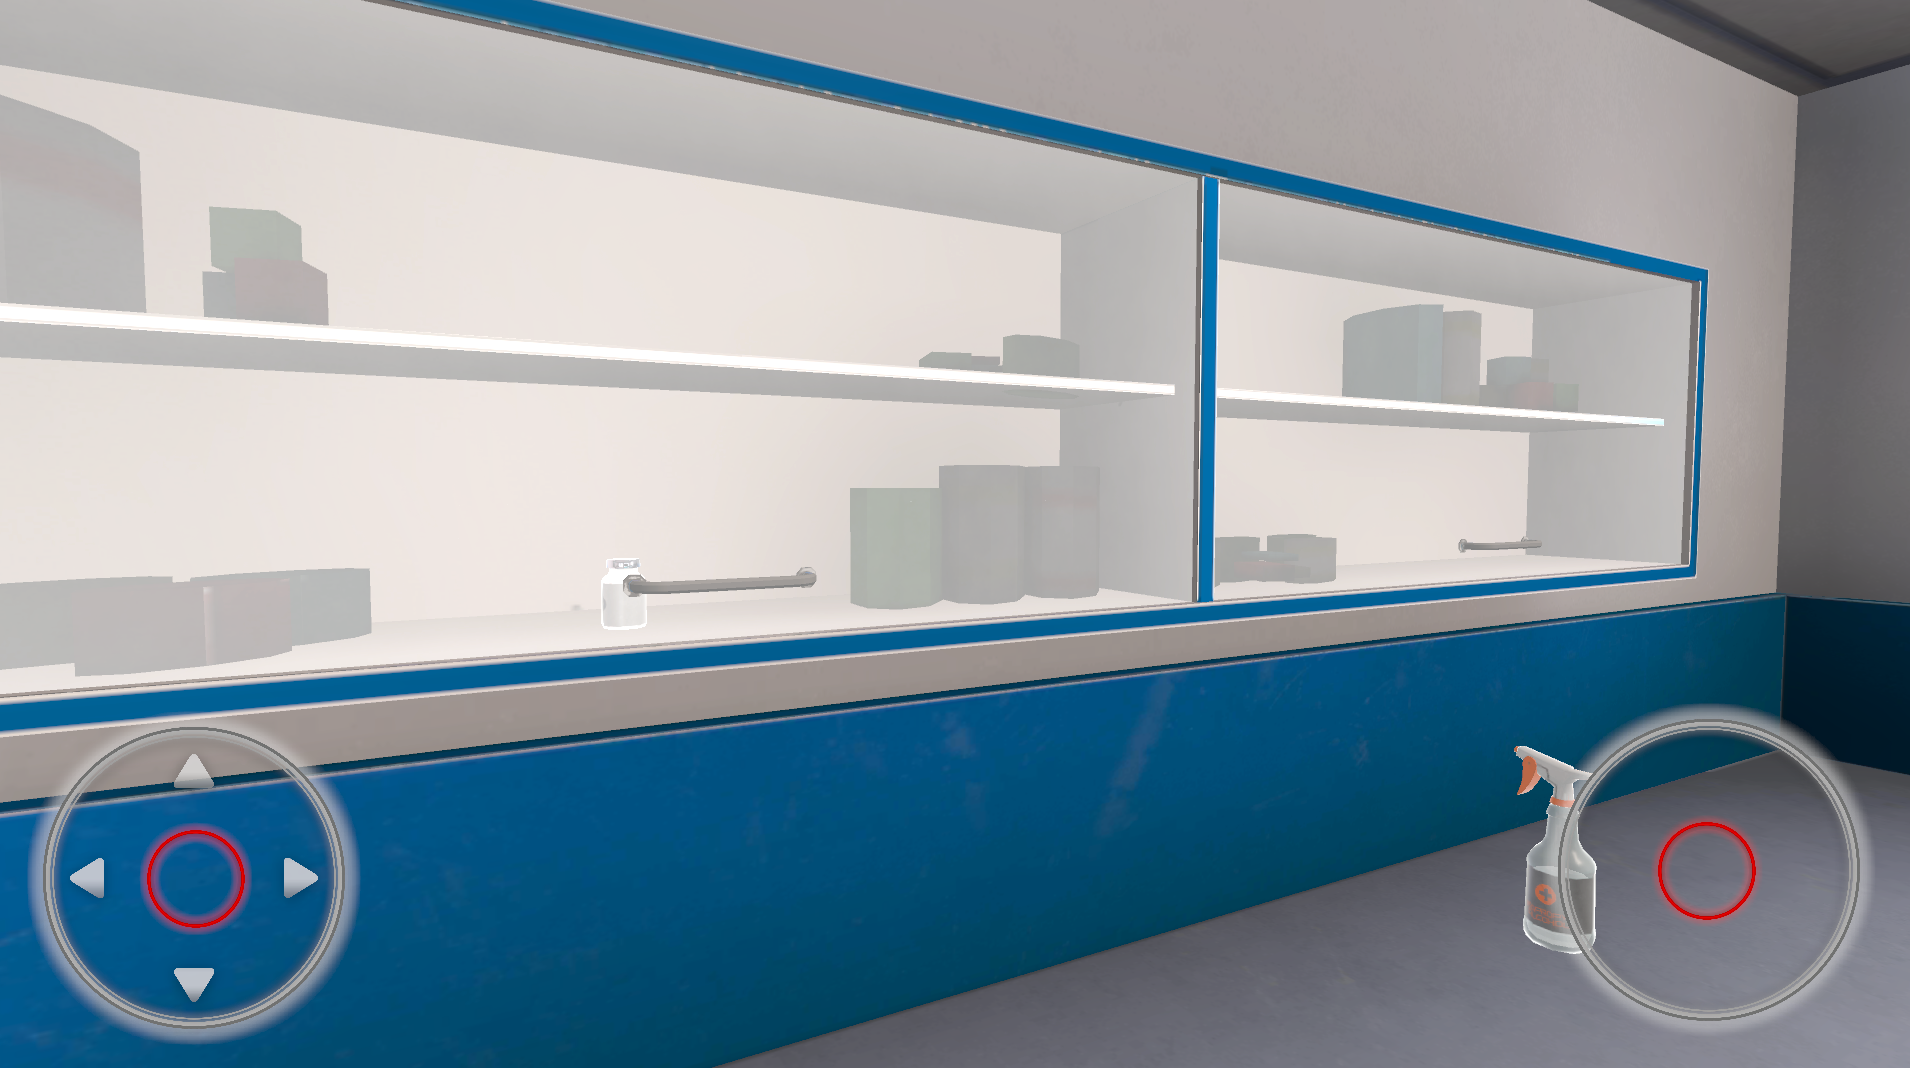
\includegraphics[width=0.65\linewidth]{Images/Tools and Medicine.png}
	\caption{Tools and Medicine}
	\label{fig:system-diagram}
\end{figure}

\subsection{Tools Grabbing}
\text{Here are some actions performed before starting.}
\subsubsection{Washing hands}
\text{Here are some actions performed before starting.}
\begin{figure}[h]
	\centering
	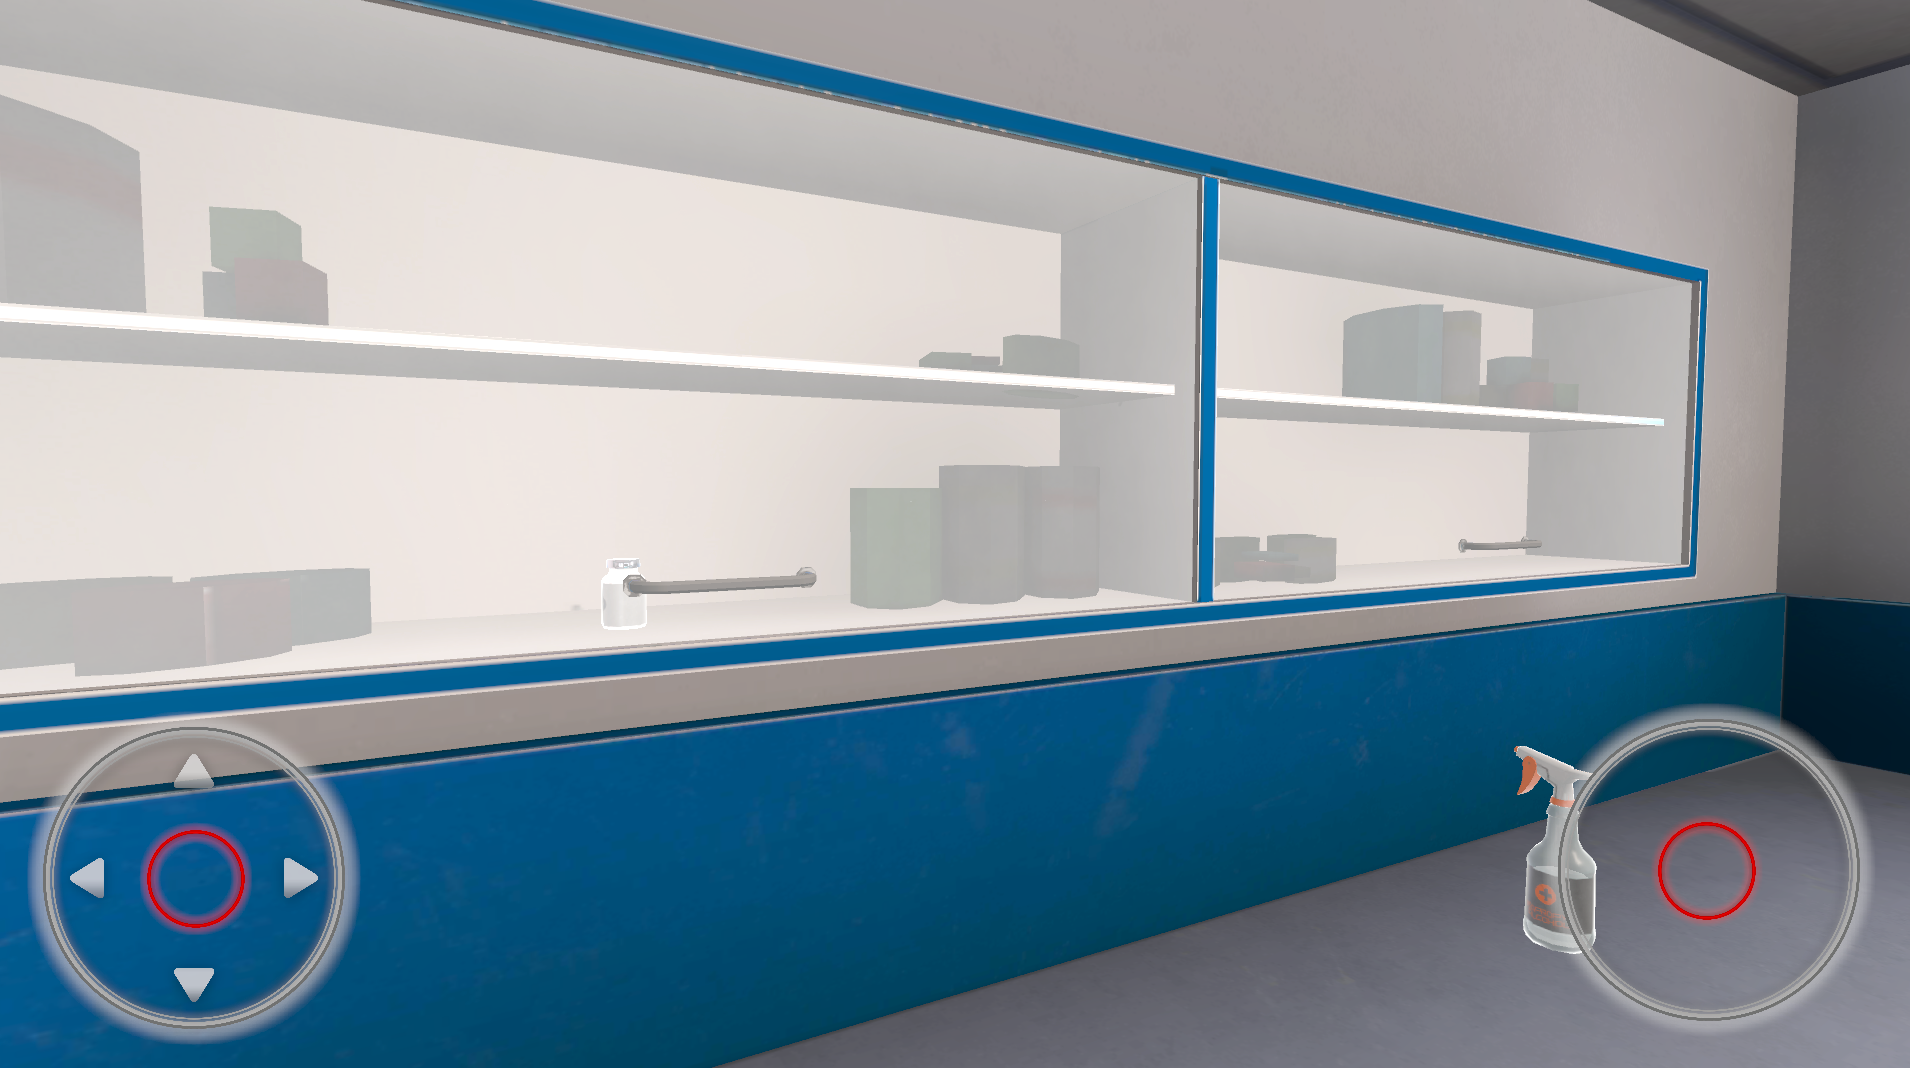
\includegraphics[width=0.65\linewidth]{Images/Tools and Medicine.png}
	\caption{Tools and Medicine}
	\label{fig:system-diagram}
\end{figure}

\subsubsection{Pour Alcohol}
\text{Here are some actions performed before starting.}
\begin{figure}[h]
	\centering
	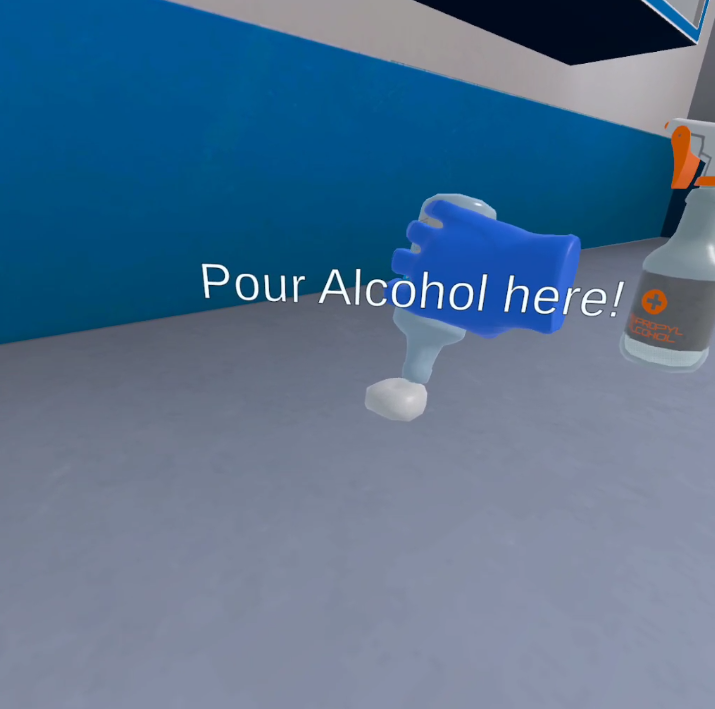
\includegraphics[width=0.65\linewidth]{Images/Pour Alcohol.png}
	\caption{Pour Alcohol}
	\label{fig:Pour-Alcohol}
\end{figure}

\subsubsection{Clean the injection site}
\text{Here are some actions performed before starting.}
\begin{figure}[h]
	\centering
	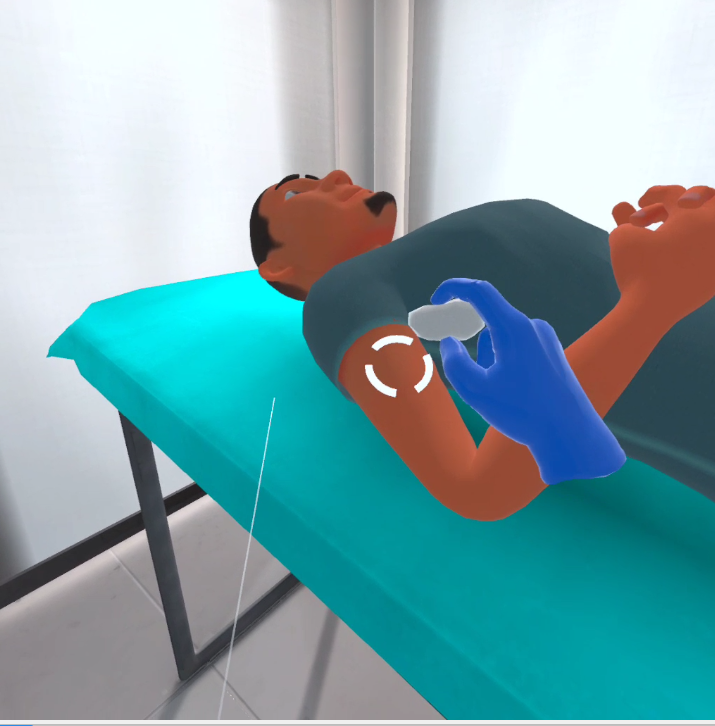
\includegraphics[width=0.65\linewidth]{Images/Clean the injection site.png}
	\caption{Clean the injection site}
	\label{fig:Clean the injection site}
\end{figure}

\subsubsection{Dispose the Cotton}
\text{Here are some actions performed before starting.}
\begin{figure}[h]
	\centering
	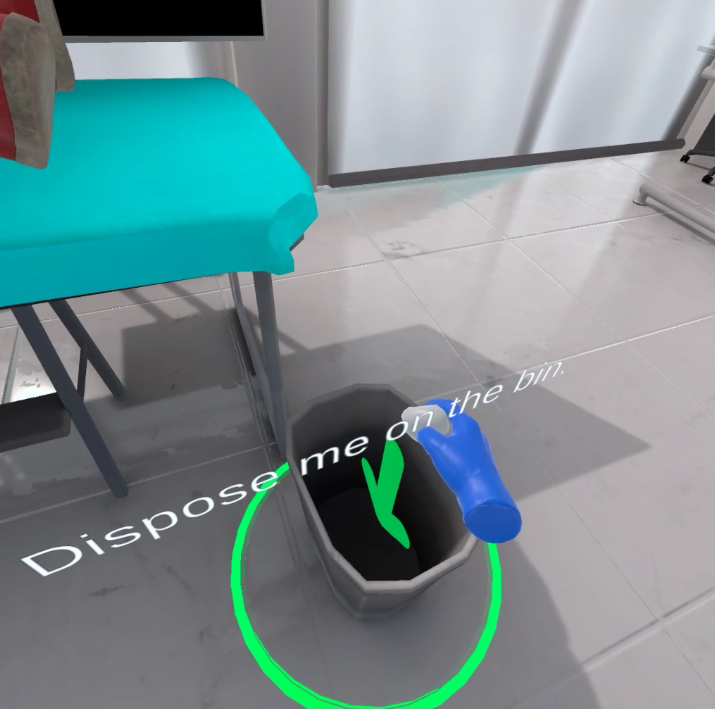
\includegraphics[width=0.65\linewidth]{Images/Dispose the Cotton.png}
	\caption{Tools and Medicine}
	\label{fig:system-diagram}
\end{figure}



\subsection{Tools Grabbing}
\text{We added some basic tools and medicines for practice.}
\subsubsection{Washing hands}
\text{Here are some actions performed before starting.}
\begin{figure}[h]
	\centering
	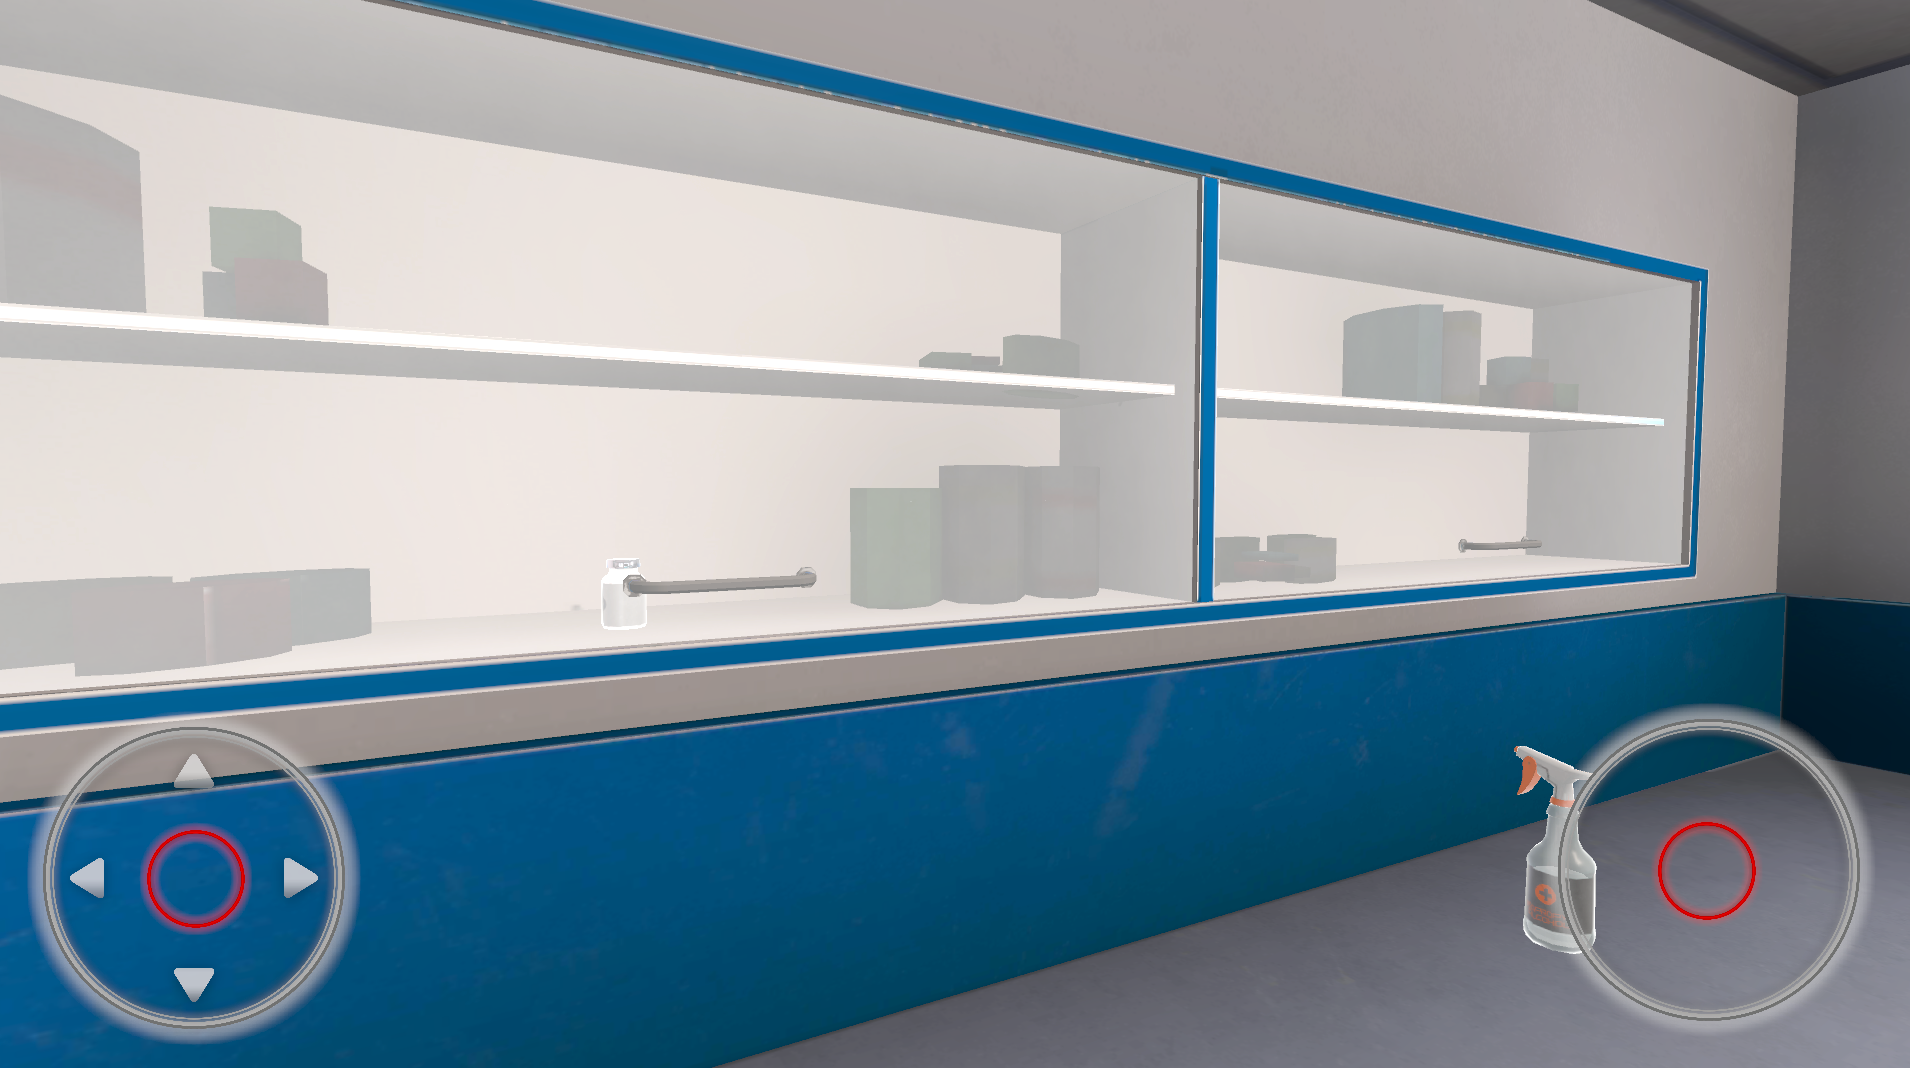
\includegraphics[width=0.65\linewidth]{Images/Tools and Medicine.png}
	\caption{Tools and Medicine}
	\label{fig:system-diagram}
\end{figure}

\subsubsection{Washing hands}
\text{Here are some actions performed before starting.}
\begin{figure}[h]
	\centering
	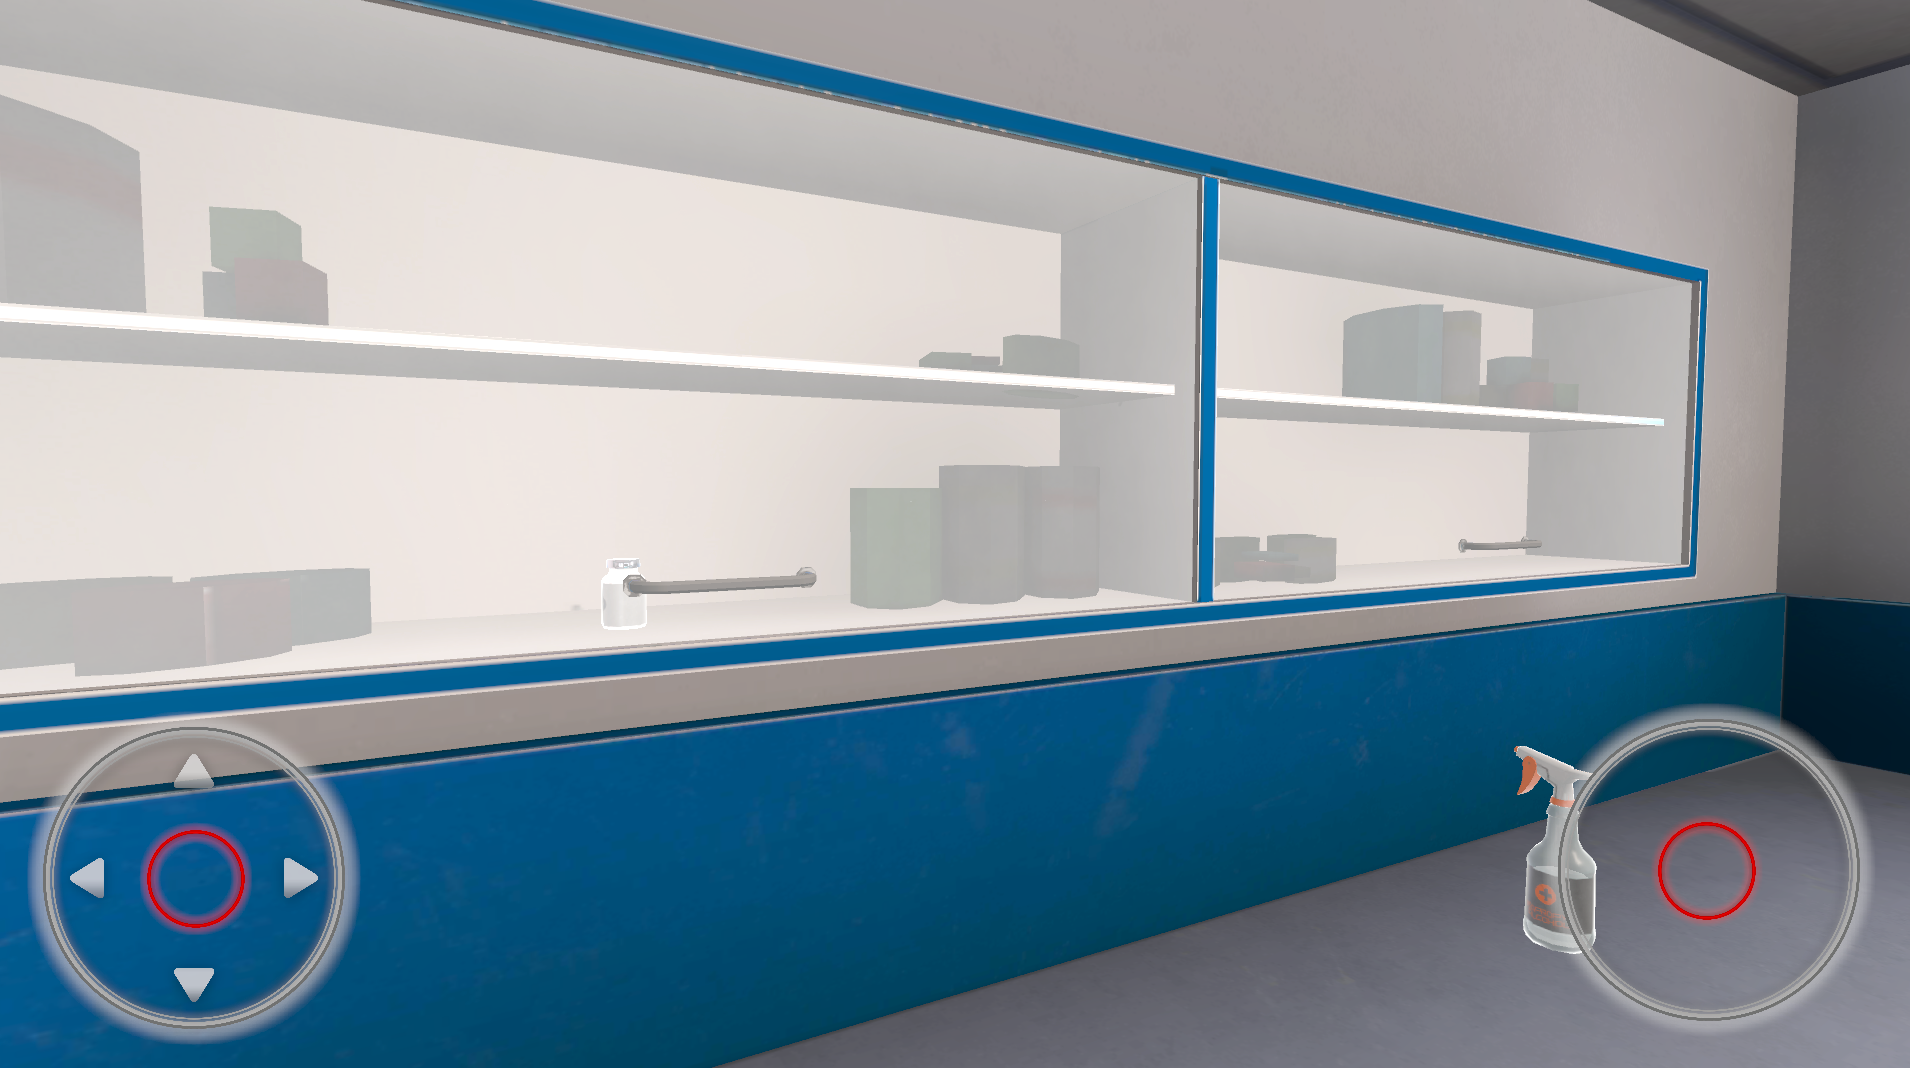
\includegraphics[width=0.65\linewidth]{Images/Tools and Medicine.png}
	\caption{Tools and Medicine}
	\label{fig:system-diagram}
\end{figure}

\subsubsection{Washing hands}
\text{Here are some actions performed before starting.}
\begin{figure}[h]
	\centering
	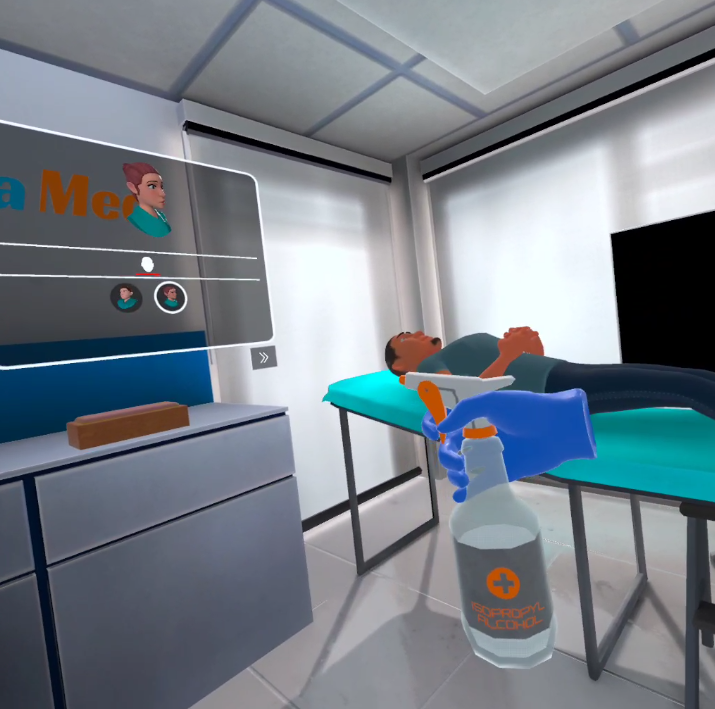
\includegraphics[width=0.65\linewidth]{Images/Washing hands.png}
	\caption{Washing hands}
	\label{fig:Washing-hands}
\end{figure}

\subsubsection{Washing hands}
\text{Here are some actions performed before starting.}
\begin{figure}[h]
	\centering
	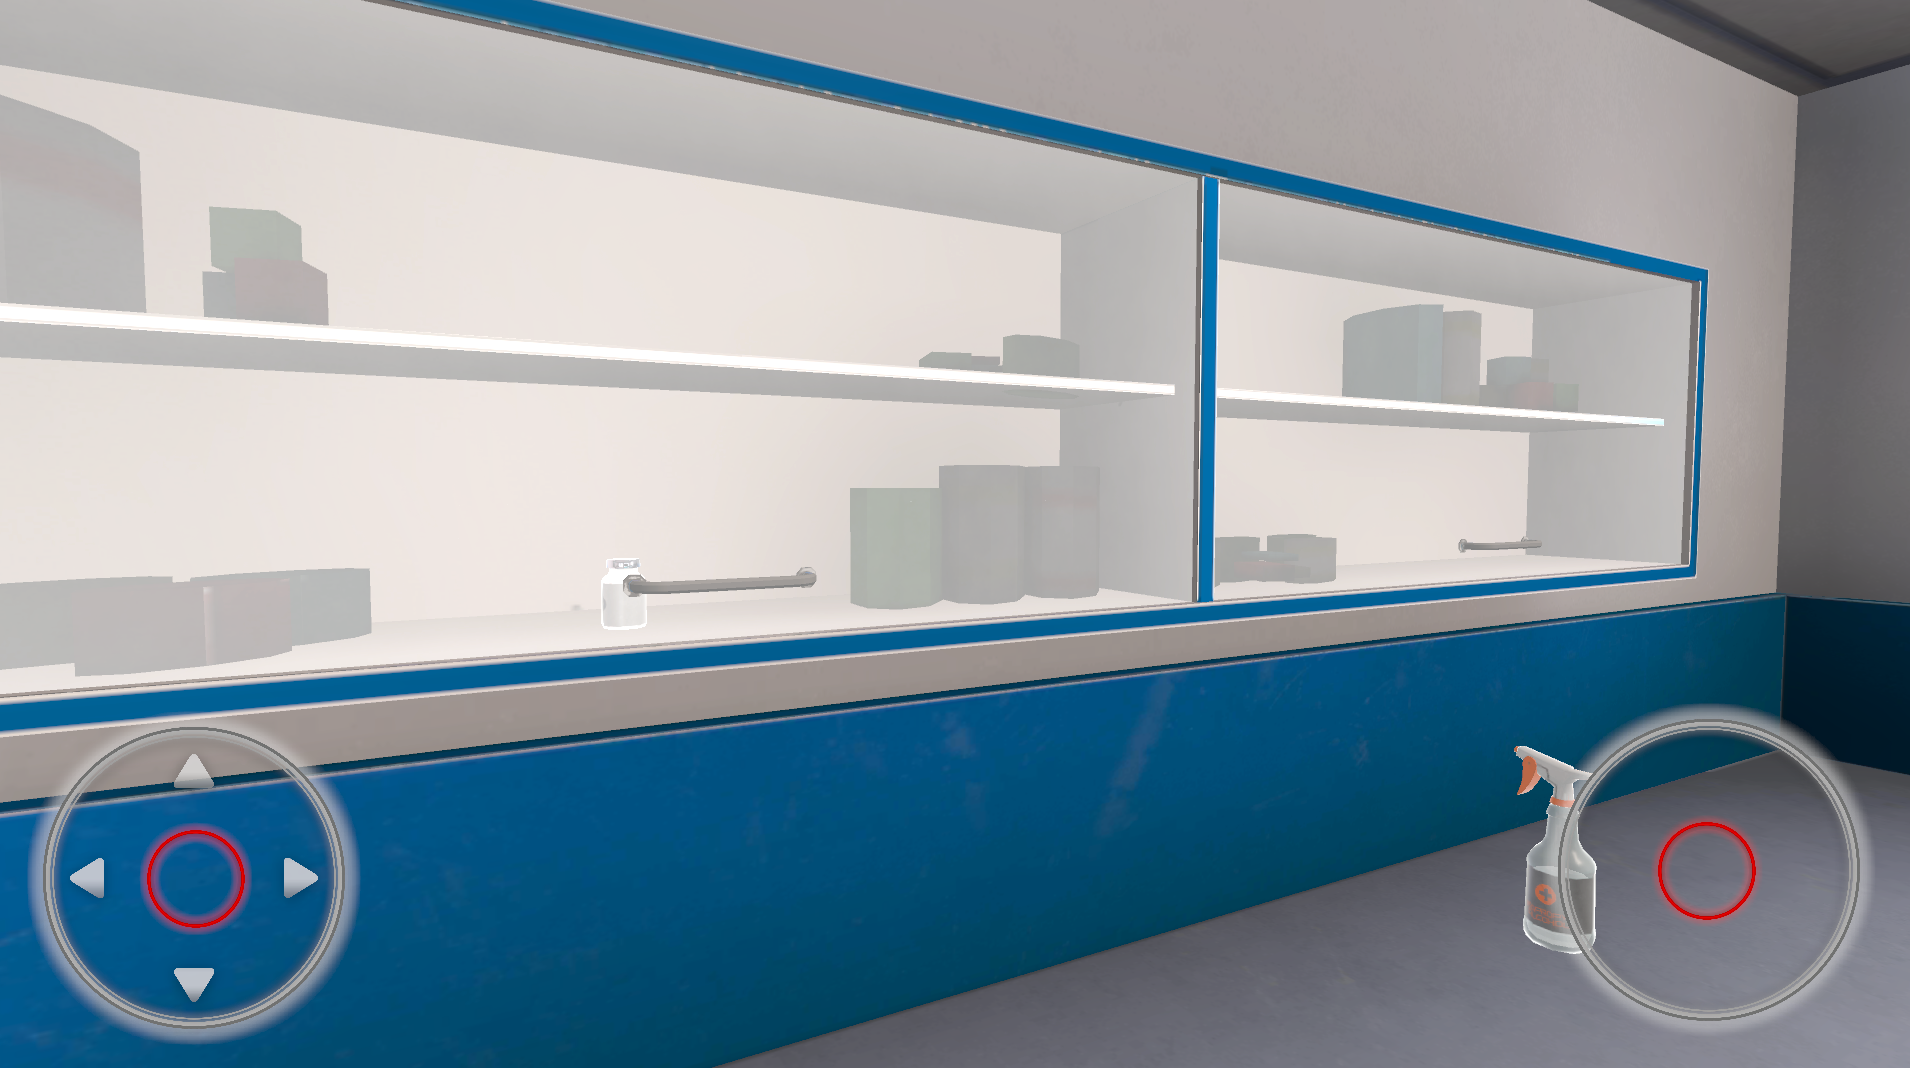
\includegraphics[width=0.65\linewidth]{Images/Tools and Medicine.png}
	\caption{Tools and Medicine}
	\label{fig:system-diagram}
\end{figure}

\subsubsection{Washing hands}
\text{Here are some actions performed before starting.}
\begin{figure}[h]
	\centering
	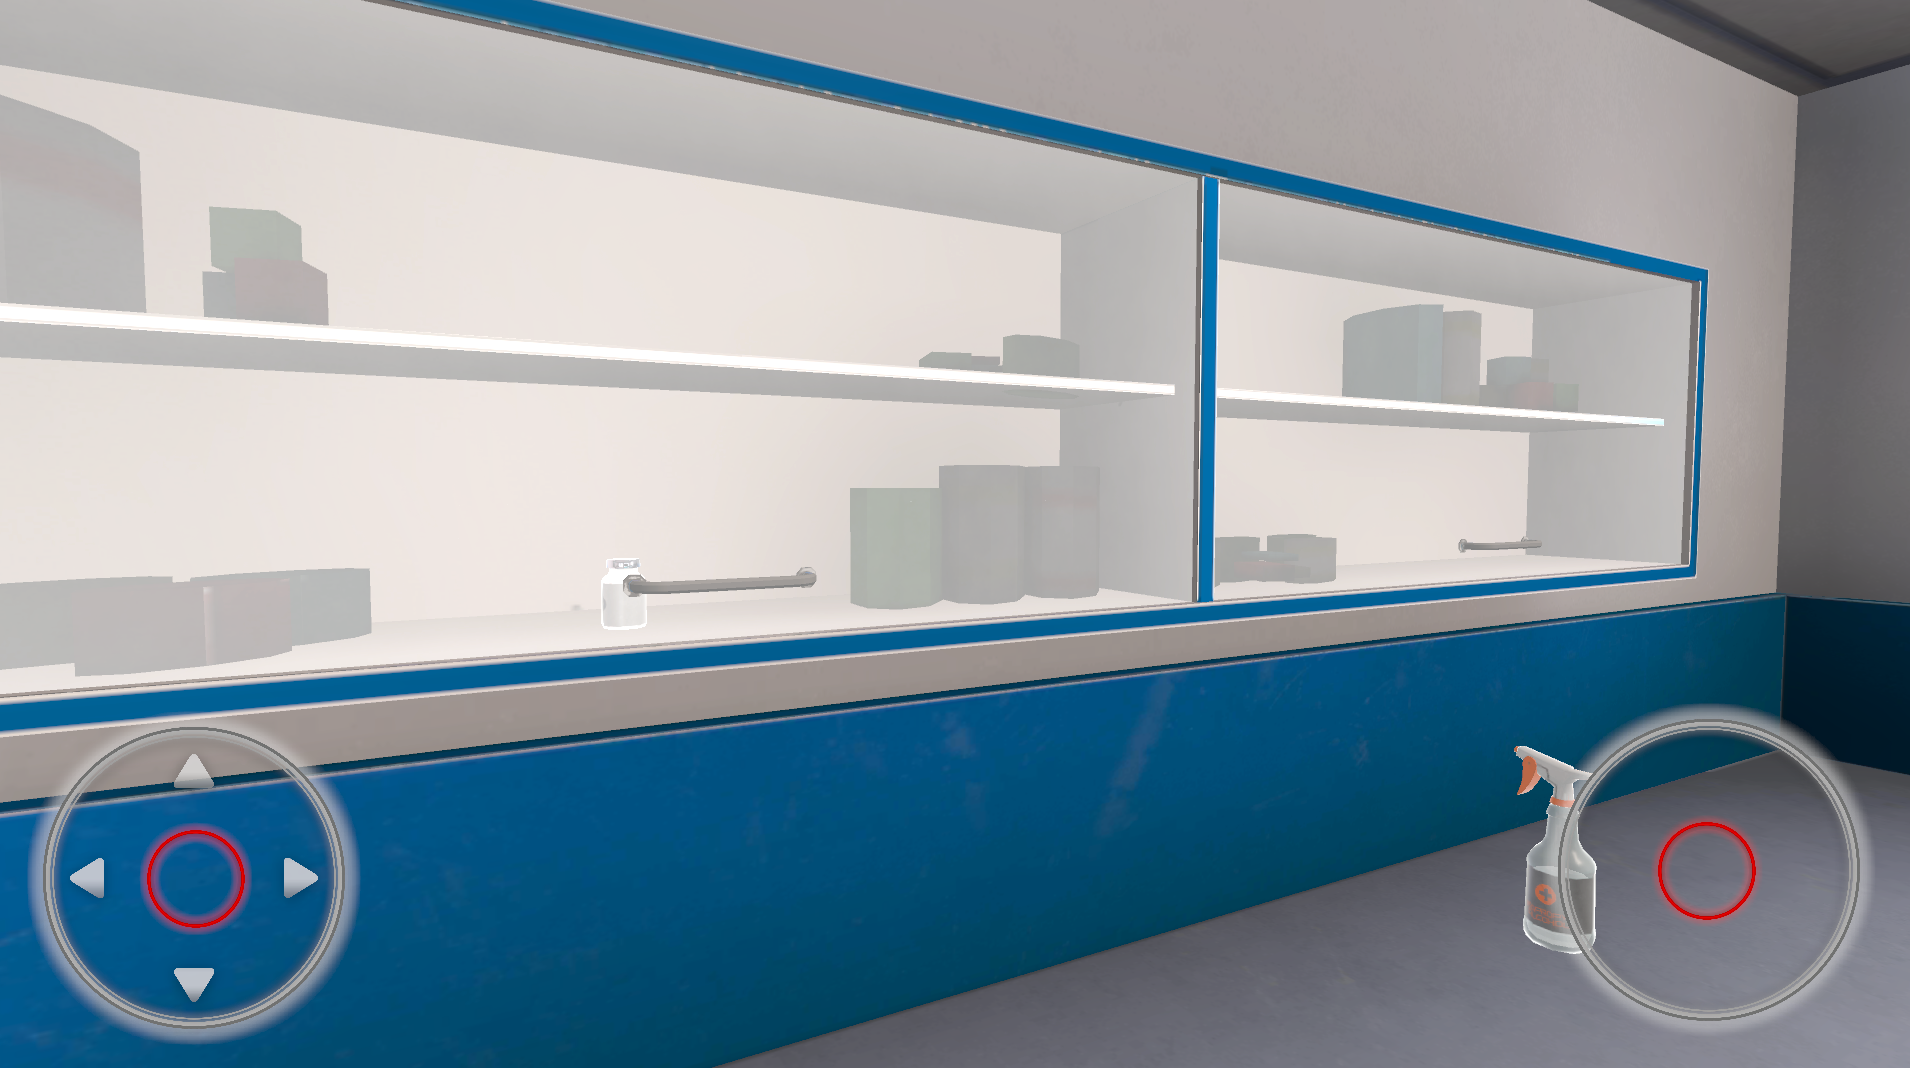
\includegraphics[width=0.65\linewidth]{Images/Tools and Medicine.png}
	\caption{Tools and Medicine}
	\label{fig:system-diagram}
\end{figure}

\subsubsection{Washing hands}
\text{Here are some actions performed before starting.}
\begin{figure}[h]
	\centering
	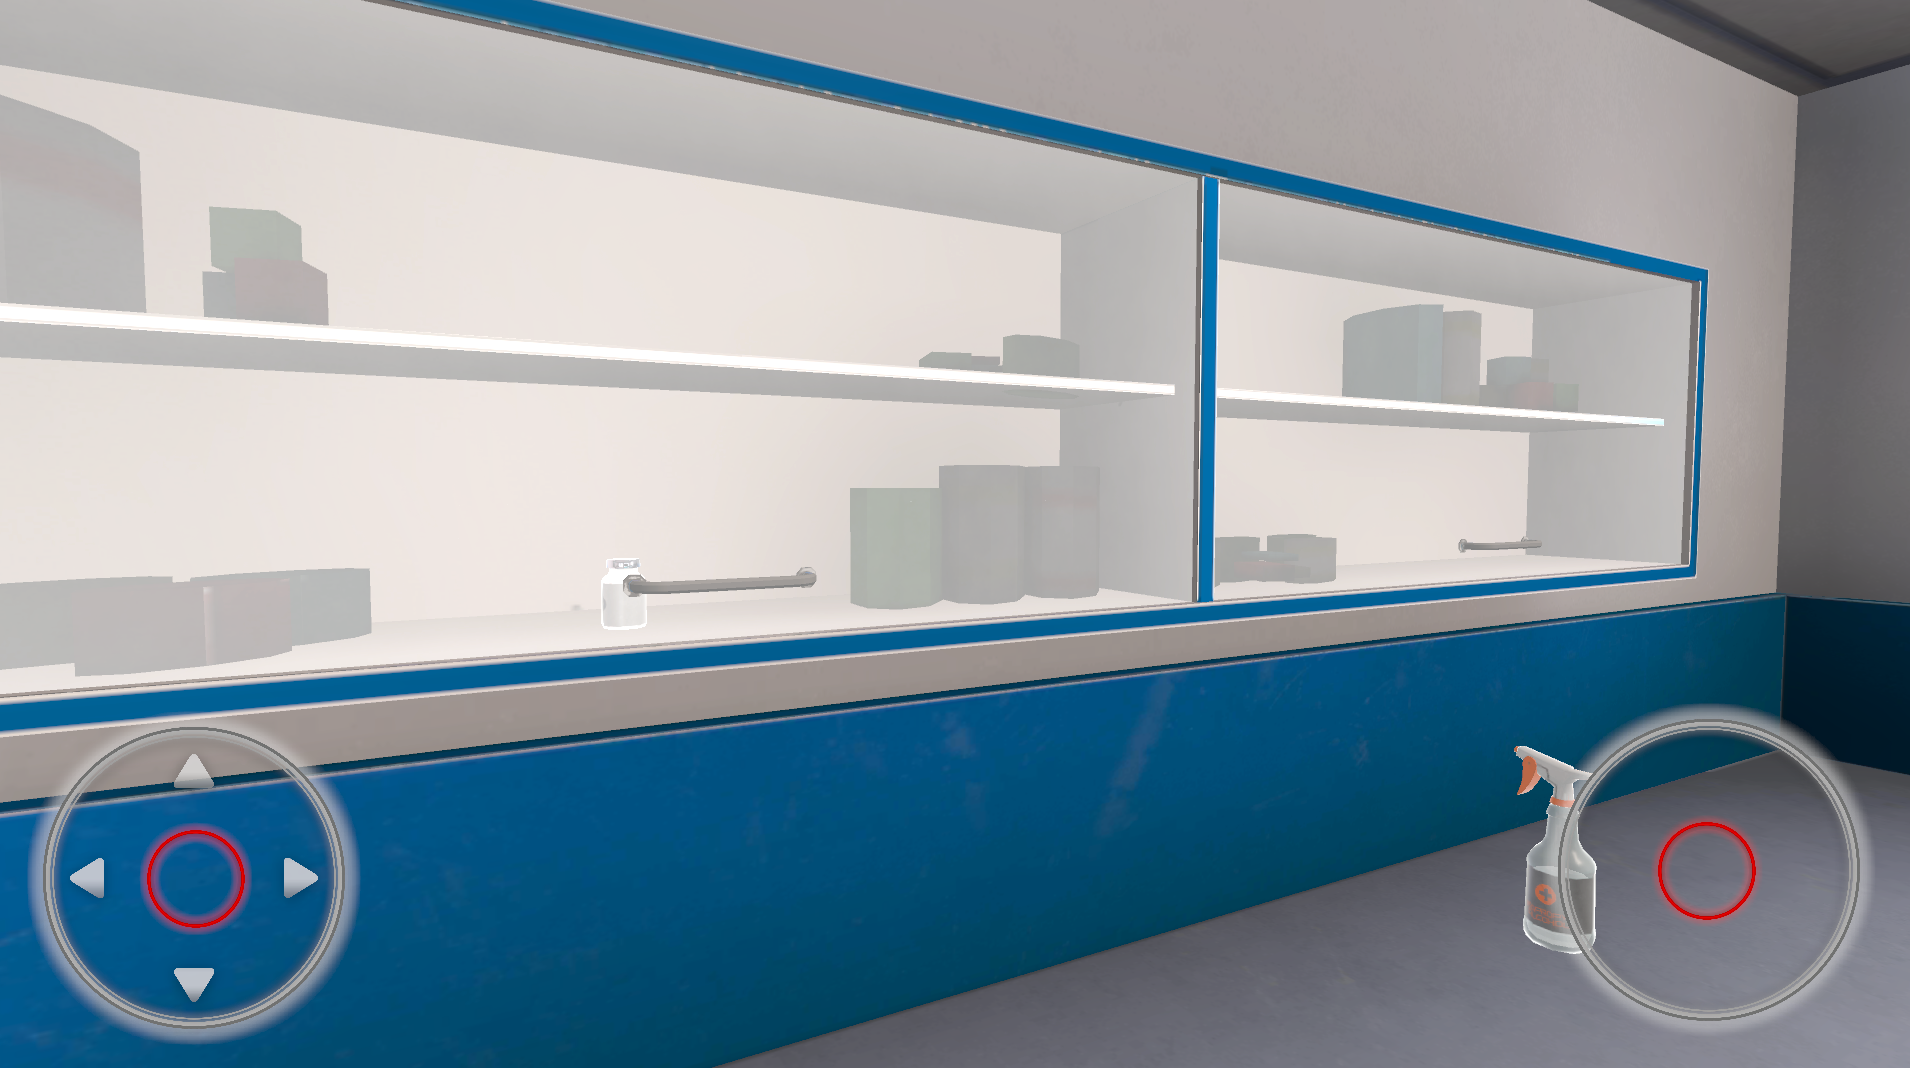
\includegraphics[width=0.65\linewidth]{Images/Tools and Medicine.png}
	\caption{Tools and Medicine}
	\label{fig:system-diagram}
\end{figure}

\section{SVN or GitHub}
We have uploaded on GitHub. Here is the GitHub link: \\
\href{https://github.com/Daudsarfraz/MetaMed}{https://github.com/Daudsarfraz/MetaMed}